\documentclass[12pt]{report}
\usepackage[utf8]{inputenc}
\usepackage[russian]{babel}
%\usepackage[14pt]{extsizes}
\usepackage{listings}

% Для листинга кода:
\lstset{ %
language=python,                 % выбор языка для подсветки (здесь это С)
basicstyle=\small\sffamily, % размер и начертание шрифта для подсветки кода
numbers=left,               % где поставить нумерацию строк (слева\справа)
numberstyle=\tiny,           % размер шрифта для номеров строк
stepnumber=1,                   % размер шага между двумя номерами строк
numbersep=5pt,                % как далеко отстоят номера строк от подсвечиваемого кода
showspaces=false,            % показывать или нет пробелы специальными отступами
showstringspaces=false,      % показывать или нет пробелы в строках
showtabs=false,             % показывать или нет табуляцию в строках
frame=single,              % рисовать рамку вокруг кода
tabsize=2,                 % размер табуляции по умолчанию равен 2 пробелам
captionpos=t,              % позиция заголовка вверху [t] или внизу [b] 
breaklines=true,           % автоматически переносить строки (да\нет)
breakatwhitespace=false, % переносить строки только если есть пробел
escapeinside={\#*}{*)}   % если нужно добавить комментарии в коде
}

% Для измененных титулов глав:
\usepackage{titlesec, blindtext, color} % подключаем нужные пакеты
\definecolor{gray75}{gray}{0.75} % определяем цвет
\newcommand{\hsp}{\hspace{20pt}} % длина линии в 20pt
% titleformat определяет стиль
\titleformat{\chapter}[hang]{\Huge\bfseries}{\thechapter\hsp\textcolor{gray75}{|}\hsp}{0pt}{\Huge\bfseries}


% plot
\usepackage{pgfplots}
\usepackage{filecontents}
\usetikzlibrary{datavisualization}
\usetikzlibrary{datavisualization.formats.functions}

\begin{document}
 
%\def\chaptername{} % убирает "Глава"
\begin{titlepage}
	\centering
	{\scshape\LARGE МГТУ им. Баумана \par}
	\vspace{3cm}
	{\scshape\Large Лабораторная работа №2\par}
	\vspace{0.5cm}	
	{\scshape\Large По курсу: "Анализ алгоритмов"\par}
	\vspace{1.5cm}
	{\huge\bfseries Алгоритмы сортировки\par}
	\vspace{2cm}
	\Large Работу выполнил: студент группы ИУ7-53Б Наместник Анастасия\par
	\vspace{0.5cm}
	\LargeПреподаватели:  Волкова Л.Л., Строганов Ю.В.\par

	\vfill
	\large \textit {Москва, 2020} \par
\end{titlepage}

\tableofcontents

\newpage
\chapter*{Введение}
\addcontentsline{toc}{chapter}{Введение}

\textbf{            		Сортировкой или упорядочением массива} называется расположение его элементов по возрастанию (или убыванию).  Для решения задачи сортировки было разработано множество алгоритмов, различающихся по трудоемкости и эффективности в связи с затрачиваемыми ими ресурсами ЭВМ. К таким алгоритмам относятся сортировка пузырьком, сортировка вставками, сортировка выбором, сортировка Шелла, сортировка расческой, быстрая сортировка и многие другие. Критерии оценки эффективности этих алгоритмов могут включать следующие параметры.
\begin{enumerate}
\item Количество шагов алгоритма, необходимых для упорядочения.
\item Количество сравнений элементов.
\item Количество перестановок, выполняемых при сортировке.
\end{enumerate}

 В рамках этой лабораторной работы будут рассмотрены следующие алгоритмы сортировки: сортировка пузырьком,  сортировка вставками и быстрая сортировка.

	Целью данной лабораторной работы является изучение, реализация и сравнительный анализ алгоритмов сортировки массивов. 

В данной лабораторной работе требуется решить пять задач.
\begin{enumerate}
\item Изучить и программно реализовать алгоритм сортировки пузырьком.
\item Изучить и программно реализовать алгоритм сортировки вставками.
\item Изучить и программно реализовать алгоритм быстрой сортировки.
\item Оценить трудоемкость вышеперечисленных алгоритмов.
\item Сделать сравнительный анализ по затрачиваемым ресурсам (времени) компьютера на реализацию каждого рассмотренного алгоритма.
\end{enumerate}


\chapter{Аналитическая часть}
 
 \section{Описание алгоритмов}
 
 Первые прототипы современных алгоритмов сортировки появились еще в XIX веке \cite{bib5}, и впоследствии сортировка стала одной из наиболее распространенных операций обработки массивов данных. Благодаря ей, ускоряется процесс решения таких задач, как:
\begin{enumerate}
\item Поиск заданного элемента в массиве.
\item Определение, имеются ли пропущенные элементы в массиве.
\item Сравнение двух массивов.
\end{enumerate}

Рассмотрим некоторые популярные алгоритмы сортировки массивов.

 \section{Сортировка пузырьком}

\textbf{Сортировка пузырьком} — один из самых известных алгоритмов сортировки. Здесь нужно последовательно сравнивать значения соседних элементов и менять числа местами, если предыдущее оказывается больше последующего. Таким образом элементы с большими значениями оказываются в конце списка, а с меньшими остаются в начале.

Идея сортировки "пузырьком" состоит в том, что все соседние элементы массива попарно сравниваются друг с другом и меняются местами в том случае, если предшествующий элемент больше (меньше) последующего. Затем процесс повторяется. Сортировка заканчивается, когда перестановок в массиве не будет.

Особенность данного алгоритма заключается в следующем: после первого завершения внутреннего цикла максимальный элемент массива размеров в N элементов всегда находится на N-ой позиции. При втором проходе, следующий по значению максимальный элемент находится на N-1 месте. И так далее. Таким образом, на каждом следующем проходе число обрабатываемых элементов уменьшается на 1 и нет необходимости «обходить» весь массив от начала до конца каждый раз.

Этот алгоритм считается учебным и почти не применяется на практике из-за низкой эффективности: он медленно работает на тестах, в которых маленькие элементы (их называют «черепахами») стоят в конце массива. Однако на нём основаны многие другие методы, например, шейкерная сортировка и сортировка расчёской.

\section{Сортировка вставками} 

\textbf{Сортировка вставками} - алгоритм сортировки, в котором элементы входной последовательности просматриваются по одному, и каждый новый поступивший элемент размещается в подходящее место среди ранее упорядоченных элементов. В начальный момент отсортированная последовательность пуста. На каждом шаге алгоритма выбирается один из элементов входных данных и помещается на нужную позицию в уже отсортированной последовательности до тех пор, пока набор входных данных не будет исчерпан. В любой момент времени в отсортированной последовательности элементы удовлетворяют требованиям к выходным данным алгоритма.
Основной цикл алгоритма начинается не с 0-го элемента а с 1-го, потому что элемент до 1-го элемента будет считаться отсортированной последовательностью (массив, состоящий из одного элемента, является отсортированным), и уже относительно этого элемента с номером 0 будут вставляться все остальные. 

На рисунке \ref{fg:ref1} представлен пример сортировки вставками.
\begin{figure}[ht!]
	\centering{
		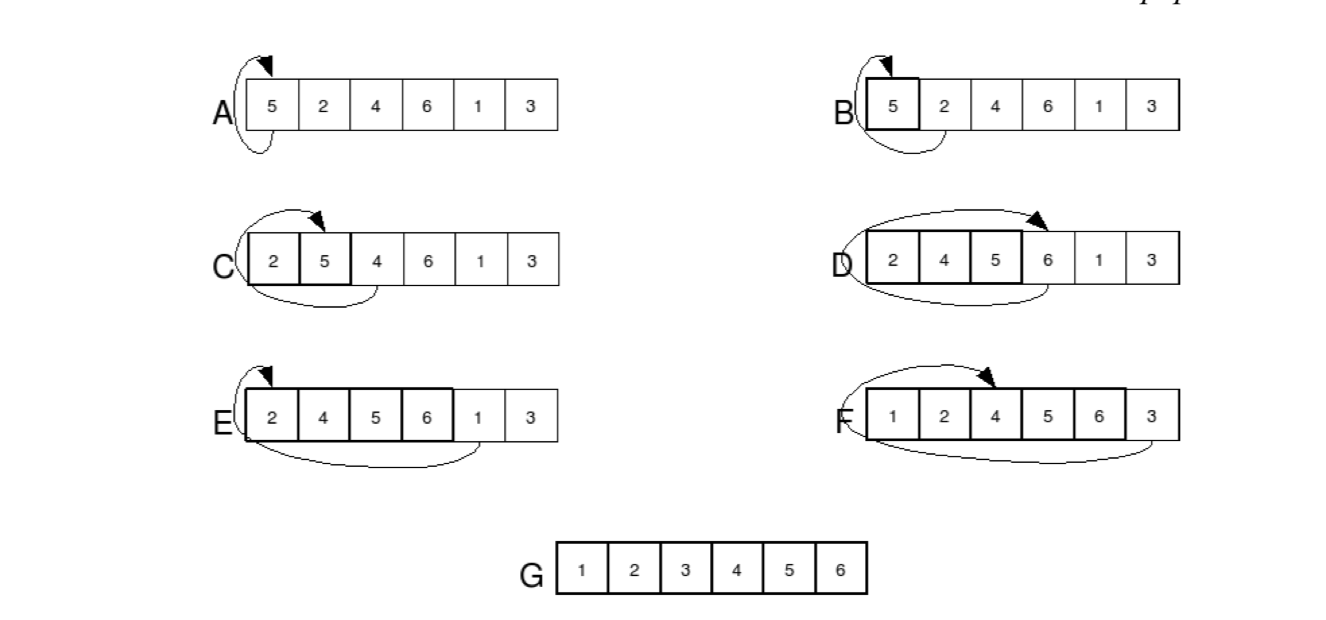
\includegraphics[scale=0.7]{pics/insert.png}
		\caption{Пример сортировки вставками}
		\label{fg:ref1}}
\end{figure}

Таким образом, суть сортировки вставками заключается в следующем.
\begin{enumerate}
\item Перебираются элементы в неотсортированной части массива.
\item Каждый элемент вставляется в отсортированную часть массива на то место, где он должен находиться.
\end{enumerate}

\section{Быстрая сортировка}

\textbf{Быстрая сортировка}, часто называемая qsort (по имени в стандартной библиотеке языка Си) — один из самых быстрых известных универсальных алгоритмов сортировки массивов. 

Общая идея алгоритма состоит в следующем.

\begin{enumerate}
\item Выбрать из массива элемент, называемый опорным. Это может быть любой из элементов массива. От выбора опорного элемента не зависит корректность алгоритма, но в отдельных случаях может сильно зависеть его эффективность.
\item Сравнить все остальные элементы с опорным и переставить их в массиве так, чтобы разбить массив на три непрерывных отрезка, следующих друг за другом: «элементы меньшие опорного», «равные» и «большие».
\item Для отрезков «меньших» и «больших» значений выполнить рекурсивно ту же последовательность операций, если длина отрезка больше единицы.
\end{enumerate}

Таким образом, алгоритм сводится к выполнению следующих трех шагов.
\begin{enumerate}
\item Выбрать элемент из массива. Назовём его опорным.
\item Разбиение: перераспределение элементов в массиве таким образом, что элементы меньше опорного помещаются перед ним, а больше или равные после.
\item Рекурсивно применить первые два шага к двум подмассивам слева и справа от опорного элемента. Рекурсия не применяется к массиву, в котором только один элемент или отсутствуют элементы.
\end{enumerate}

\section{Вывод}

Были рассмотрены основные теоретические сведения о трех распространенных алгоритмах сортировки массивов: сортировка пузырьком, сортировка вставками и быстрая сортировка, - которые в дальнейшем потребуются при разработке программного продукта.  

\chapter{Конструкторская часть}

В данном разделе будут представлены схемы алгоритмов сортировки массивов.

\section{Сортировка пузырьком}


На рисунке 2.1 представлена схема алгоритма сортировки пузырьком.

\begin{center}
		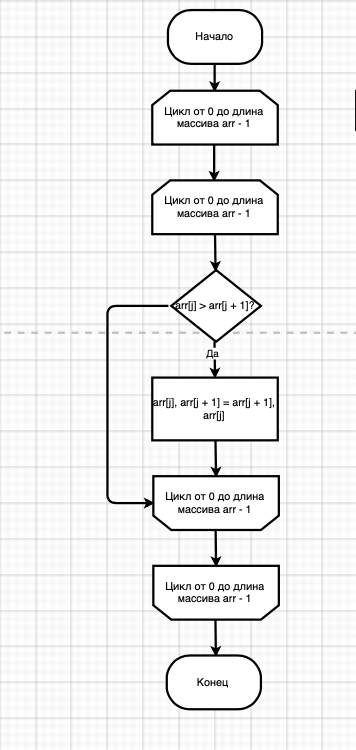
\includegraphics[scale=0.8]{schema/BubbleSort.png}
		
			Рис 2.1: Схема алгоритма сортировки пузырьком
\end{center}

На листинге 2.1 представлен псевдокод алгоритма.

\begin{lstlisting}[label=some-code,caption=Псевдокод алгоритма сортировки пузырьком]
function bubbleSort(a):
  for i = 0 to n - 2
    for j = 0 to n - 2
      if a[j] > a[j + 1]
        swap(a[j], a[j + 1])
\end{lstlisting}

\newpage
\section{Сортировка вставками}

На рисунке 2.2 представлена схема алгоритма сортировки вставками.

\begin{center}
		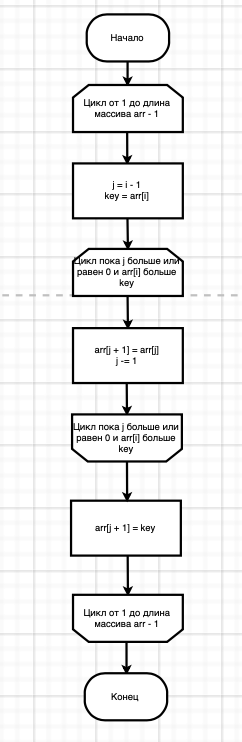
\includegraphics[scale=1.2]{schema/InsertSort.png}
		
			Рис 2.2: Схема алгоритма сортировки вставками
\end{center}

На листинге 2.2 представлен псевдокод алгоритма, где A — сортируемый массив, а low и high — соответственно, нижняя и верхняя границы сортируемого участка этого массива (предполагается, что неописанная функция partition возвращает индекс опорного элемента).

\begin{lstlisting}[label=some-code,caption=Псевдокод алгоритма быстрой сортировки]
algorithm quicksort(A, low, high) is
    if low < high then
        p := partition(A, low, high)
        quicksort(A, low, p - 1)
        quicksort(A, p + 1, high)\end{lstlisting}

\newpage
\section{Быстрая сортировка}

На рисунках 2.3 - 2.4 - 2.5 представлена схема алгоритма быстрой сортировки.

\begin{center}
		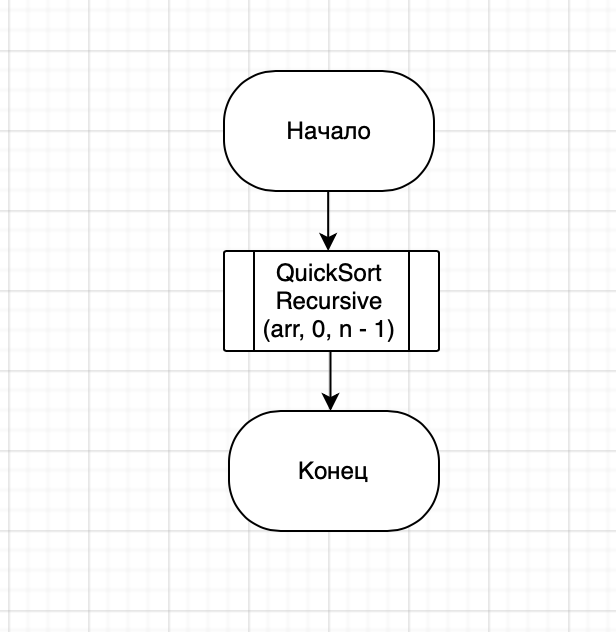
\includegraphics[scale=0.8]{schema/QuickSort.png}
		
			Рис 2.3: Схема алгоритма быстрой сортировки (часть 1)
\end{center}

\begin{center}
		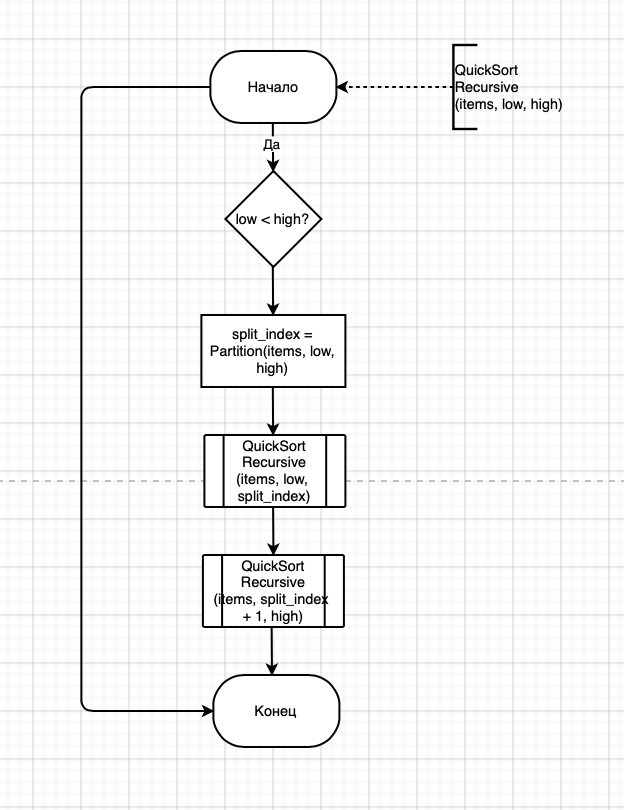
\includegraphics[scale=1.1]{schema/QuickSortRec.png}
		
			Рис 2.4: Схема алгоритма быстрой сортировки (часть 2)
\end{center}

\begin{center}
		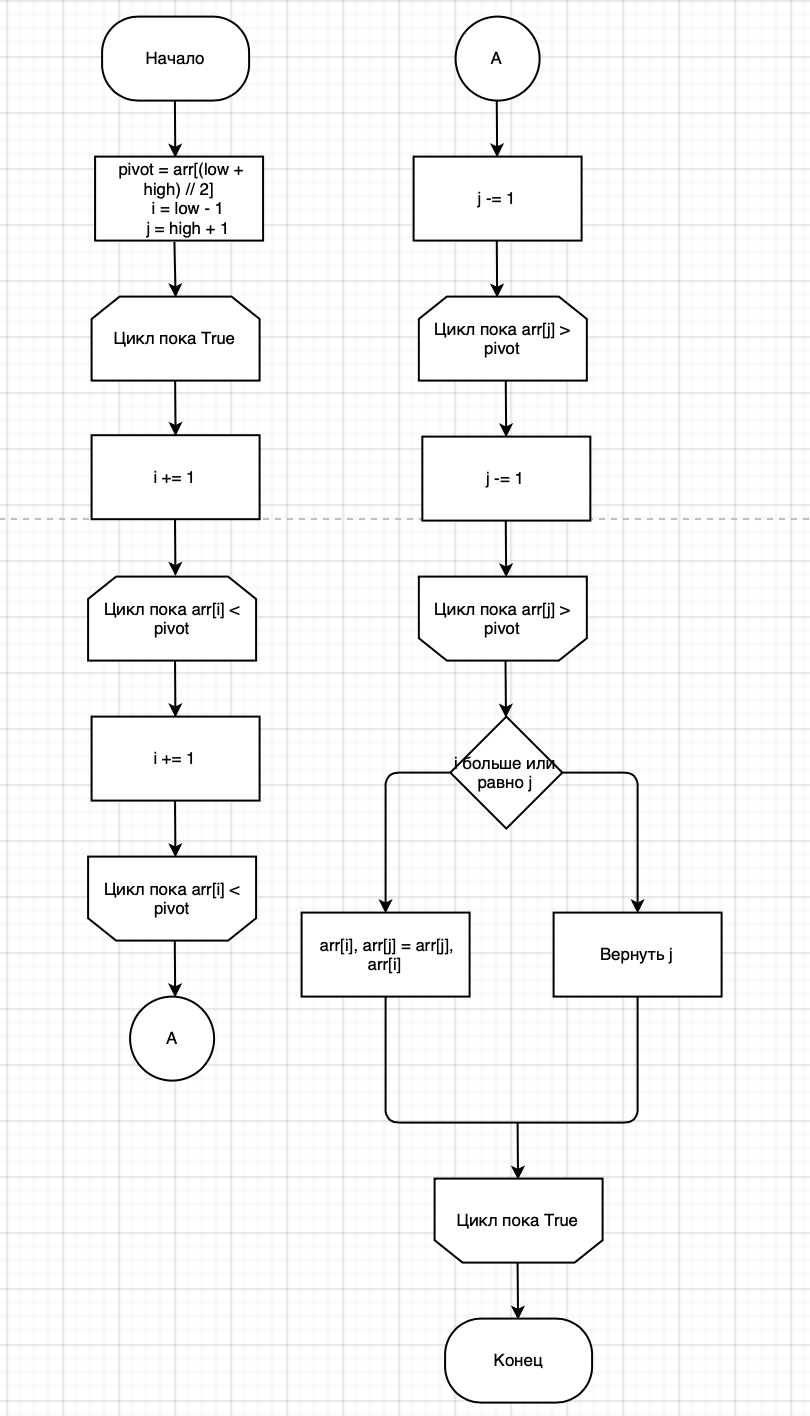
\includegraphics[scale=0.7]{schema/Partition.png}
		
			Рис 2.5: Схема алгоритма быстрой сортировки (часть 3)
\end{center}

\section{Вывод}
В данном разделе были рассмотрены схемы трех алгоритмов: стандартного алгоритма умножения матриц, алгоритма Винограда умножения матриц и алгоритма Винограда умножения матриц с оптимизациями. Из полученных данных можно отметить, что объем кода растет от стандартного алгоритма к оптимизированному алгоритму Винограда, что объясняется использованием дополнительных переменных и структур данных в алгоритме Винограда умножения матриц.

\chapter{Технологическая часть}
\section{Выбор языка программирования}
В данной лабораторной работе использовался язык программирования - python (3.8.3) \cite{bib1} в целях упрощения работы со структурами и визуализацией данных сравнительных анализов, а также из-за наличия опыта работы с данным языком программирования. В качестве интегрированной среды разработки использовался интерпретатор python - IDLE  \cite{bib2}. Для замеров процедурного времени использовалась функция process\_time() библиотеки time \cite{bib3}.  Для генерации матрицы использовалась функция randint() модуля random \cite{bib4}.

\section{Сведения о модулях программы}
Программа состоит из следующих модулей:
\begin{itemize}
	\item sort.py - главный файл программы;
	\item time\_test.py - файл с замерами временнных характеристик.
\end{itemize}

\begin{lstlisting}[label=some-code,caption=Подпрограмма алгоритма сортировки "пузырьком"]
def BubbleSort(arr, n):
    for i in range(n - 1):
        for j in range(n - 1):
            if arr[j] > arr[j + 1]:
                arr[j], arr[j + 1] = arr[j + 1], arr[j]
    return arr            

\end{lstlisting}

\begin{lstlisting}[label=some-code,caption=Подпрограмма алгоритма сортировки вставками]
def InsertSort(arr, n):
    for i in range(1, n):
        j = i - 1 
        key = arr[i]
        while j >= 0 and arr[j] > key:
            arr[j + 1] = arr[j]
            j -= 1
        arr[j + 1] = key
    
    return arr
\end{lstlisting}

\begin{lstlisting}[label=some-code,caption=Подпрограмма быстрой сортировки]
def QuickSort(arr, n):  

    QuickSortRecursive(arr, 0, n - 1)
  
    return arr
\end{lstlisting}

\begin{lstlisting}[label=some-code,caption=Подпрограмма сравнения элементов с выбранным опорным]
def Partition(arr, low, high): 
    pivot = arr[(low + high) // 2]
    i = low - 1
    j = high + 1
    while True:
        i += 1
        while arr[i] < pivot:
            i += 1

        j -= 1
        while arr[j] > pivot:
            j -= 1

        if i >= j:
            return j

         arr[i], arr[j] = arr[j], arr[i]
\end{lstlisting}

\begin{lstlisting}[label=some-code,caption=Подпрограмма создания массива]
def CreateArray(n):
    arr = []
    for i in range(n):
        arr.append(int(input()))
    return arr

\end{lstlisting}

\begin{lstlisting}[label=some-code,caption=Подпрограмма создания массива с использованием функции randint модуля random  \cite{bib4}]
def CreateArrayRandom(n):
    return [randint(0, 100) for i in range(n)]
\end{lstlisting}

\section{Тесты}

В данном разделе будут представлены тесты.

\begin{enumerate}
	\itemПри массиве arr = [1, 3, 5, 2, 4] длиной n = 5
	Сортировка пузырьком: 1 2 3 4 5
	Сортировка вставками: 1 2 3 4 5
	Быстрая сортировка: 1 2 3 4 5
	\itemПри массиве arr = [10, 9, 8, 7, 6, 5, 1, 2, 3, 4] длиной n = 10
	Сортировка "пузырьком": 1 2 3 4 5 6 7 8 9 10
	Сортировка вставками:  2 3 4 5 6 7 8 9 10
	Быстрая сортировка:  2 3 4 5 6 7 8 9 10
	\itemПри массиве arr = [1] длиной n = 1
	Сортировка "пузырьком": 1
	Сортировка вставками: 1
	Быстрая сортировка: 1 

\end{enumerate}

\section{Вывод}
В технологической части были представлены модули программы, листинги кода и тестов к программе, а также обусловлен выбор языка программирования и приведены использовавшиеся в ходе работы инструменты.


\chapter{Исследовательская часть}

\section{Результат замеров времени выполнения всех алгоритмов} 

Сравним временные показатели работы каждого из рассматриваемых четырех алгоритмов при длине массива от 5 до 20 чисел. Для этого установим количество итераций (повторений вызова процедуры) iter и воспользуемся библиотекой time для замера времени выполнения каждого алгоритма по iter раз. Возьмем iter = 100 и следующие массивы.
\begin{enumerate}
\item 1, 3, 2, 4, 5
\item 10, 9, 8, 7, 6, 5, 1, 2, 3, 4
\item 10, 1, 3, 2, 4, 5, 6, 8, 7, 9, 12, 11, 15, 13, 14
\item  1, 2, 3, 4, 5, 10, 9, 8, 7, 6, 5, 11, 13, 12, 14, 15, 20, 19, 16, 18, 17
\end{enumerate}

Время выполнения алгоритмов сортировки массивов довольно мало, поэтому, чтобы оценить его, следует взять среднее арифметическое от времени, за которое процедура отработает установленные iter раз. 

\section{Случайная выборка}

На рисунке 4.1 показана работа алгоритмов сортировки массивов при случайной выборке.

\begin{center}
		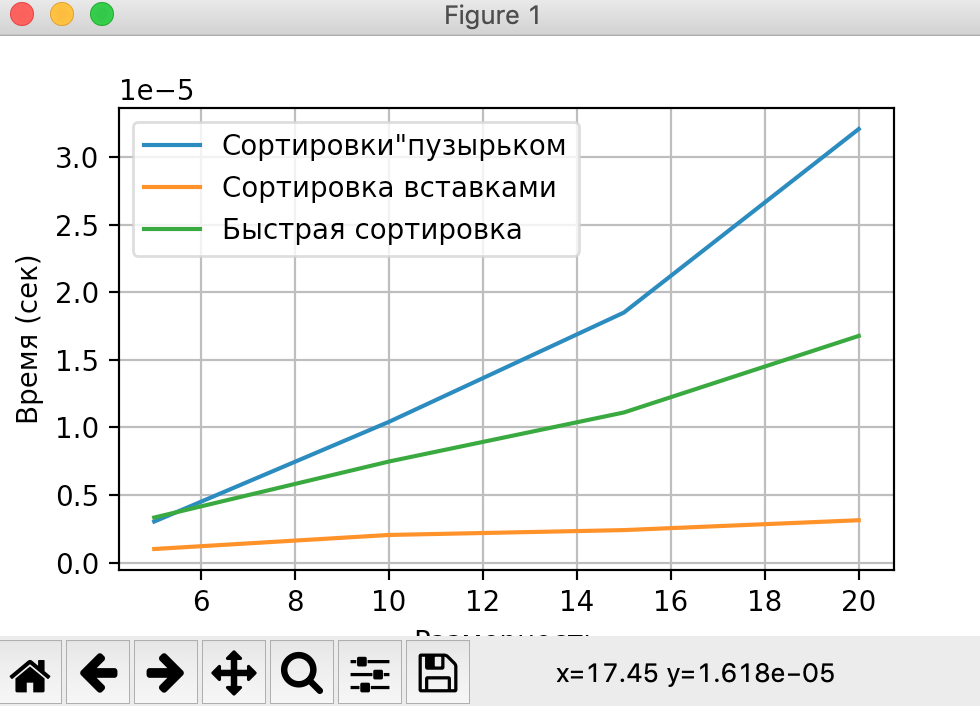
\includegraphics[scale=0.6]{pics/Time.png}
		
			Рис 4.1: Сравнение времени выполнения алгоритмов (случайная выборка)
\end{center}

В качестве примера в таблице 4.1 представлены временные характеристики всех алгоритмов при размере массива от 5 до 20 чисел.

\begin{center}
	\centering
	\caption{Сравнительная таблица времени выполнения (сек.) всех алгоритмов при случайной выборке}
	\begin{tabular}{|c c c c|}
		\hline
		Разм. алгоритма & Пузырек & Вставки & Быстрая сортировка  \\ [0.5ex] 
 		\hline\hline
		5 & 0.00000302 & 0.00000107 & 0.0000035\\
 		\hline
 		10 & 0.00001044 & 0.0000019 & 0.0000082\\
 		\hline
 		15 & 0.00001979 & 0.0000025 & 0.0000118\\
 		\hline
		20 & 0.00003753 & 0.0000040 & 0.0000172\\
		\hline
		\end{tabular}
\end{center} 

\newpage
\section{Лучший случай}

Лучшим случаем будем считать ситуацию, когда массив изначально отсортирован. Для сравнительного анализа возьмем следующие массивы.
\begin{enumerate}
\item 1, 3, 2, 4, 5
\item 1, 3, 2, 4, 5, 6, 7, 8, 9, 10
\item 1, 3, 2, 4, 5, 6, 7, 8, 9, 10, 11, 12, 13, 14, 15
\item 1, 3, 2, 4, 5, 6, 7, 8, 9, 10, 11, 12, 13, 14, 15, 16, 17, 18, 19, 20
\end{enumerate}

На рисунке 4.3 показана работа алгоритмов сортировки массивов при лучшем случае.


\begin{center}
		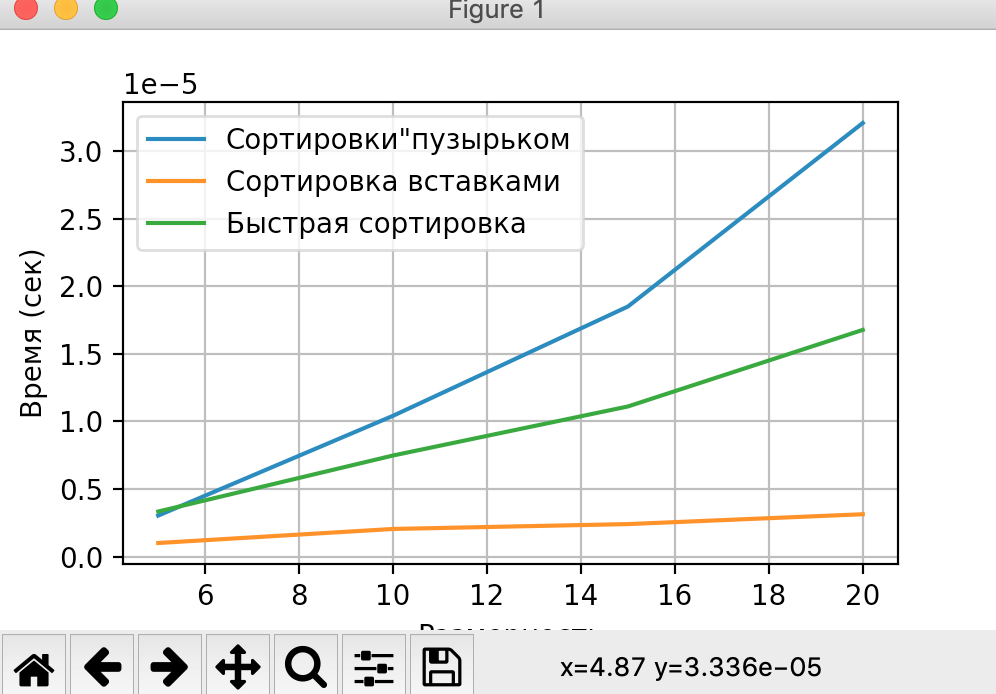
\includegraphics[scale=0.6]{pics/Best.png}
		
			Рис 4.2: Сравнение времени выполнения алгоритмов (лучший случай)
\end{center}

В качестве примера в таблице 4.2 представлены временные характеристики всех алгоритмов при размере массива от 5 до 20 чисел.

\begin{tabular}{|c c c c|}
		\hline
		Разм. алгоритма & Пузырек & Вставки & Быстрая сортировка  \\ [0.5ex] 
 		\hline\hline
		5 & 0.00000284 & 0.0000009 & 0.0000032\\
 		\hline
 		10 & 0.0000089 & 0.0000016 & 0.00000703\\
 		\hline
 		15 & 0.0000182 & 0.0000024 & 0.00001107\\
 		\hline
		20 & 0.0000317 & 0.0000031 & 0.00001539\\
		\hline
		\end{tabular}
\end{center} 

\newpage
\section{Худший случай}

Худшим случаем будем считать ситуацию, когда массив изначально отсортирован в обратном порядке. Для сравнительного анализа возьмем следующие массивы.
\begin{enumerate}
\item 5, 4, 3, 2, 1
\item 10, 9, 8, 7, 6, 5, 4, 3, 2, 1
\item 15, 14, 13, 12, 11, 10, 9, 8, 7, 6, 5, 4, 3, 2, 1
\item 20, 19, 18, 17, 16, 15, 14, 13, 12, 11, 10, 9, 8, 7, 6, 5, 4, 3, 2, 1
\end{enumerate}

На рисунке 4.3 показана работа алгоритмов сортировки массивов при худшем случае.

\begin{center}
		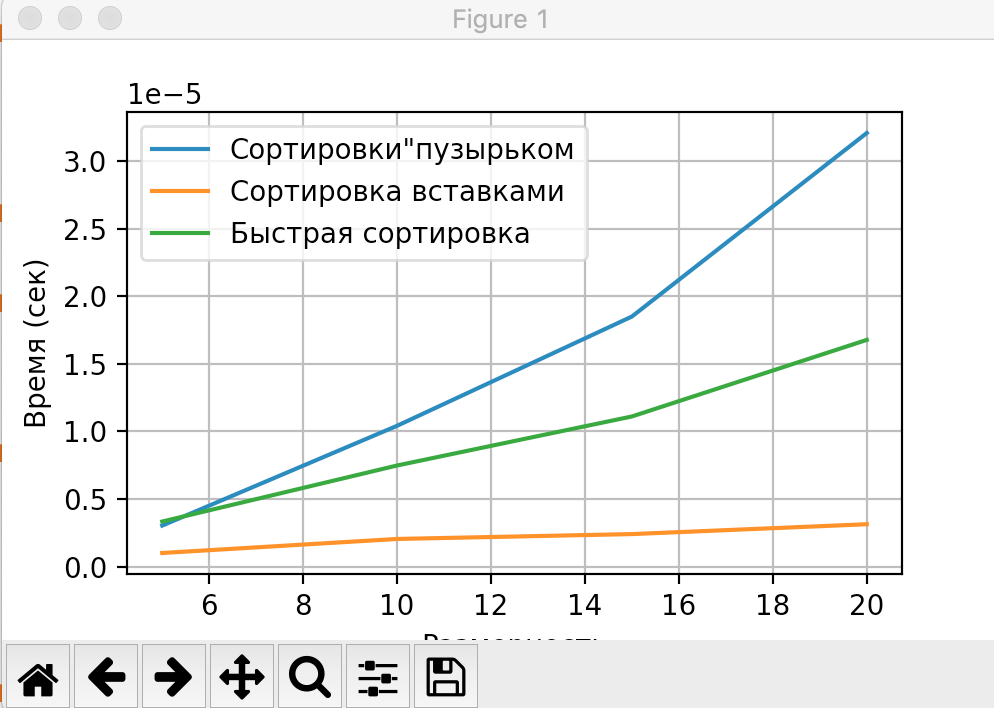
\includegraphics[scale=0.6]{pics/Worst.png}
		
			Рис 4.3: Сравнение времени выполнения алгоритмов (худший случай)
\end{center}

В качестве примера в таблице 4.3 представлены временные характеристики всех алгоритмов при размере массива от 5 до 20 чисел.

\begin{tabular}{|c c c c|}
		\hline
		Разм. алгоритма & Пузырек & Вставки & Быстрая сортировка  \\ [0.5ex] 
 		\hline\hline
		5 & 0.00000284 & 0.0000099 & 0.0000032\\
 		\hline
 		10 & 0.0000090 & 0.0000017 & 0.00000722\\
 		\hline
 		15 & 0.0000189 & 0.0000024 & 0.00001109\\
 		\hline
		20 & 0.0000326 & 0.0000031 & 0.00001541\\
		\hline
		\end{tabular}
\end{center} 

\section{Сравнительный анализ алгоритмов}

Введем модель вычислений трудоемкости алгоритма.
Пусть трудоемкость 1 у следующих базовых операций: +, -, *, /, =, ==, !=, <, <=, >, >=. Трудоемкость цикла: f цикла = f иниц + f сравн + N итер(f тела +
fинкрем + fсравн ).Трудоемкость условного перехода 1.


Алгоритм сортировки пузырьком обладает трудоемкостью \ref{eq:ref1}.

\begin{equation}
	N^2 * \left[ 
	\begin{array}{c} 
	$4 л.с.$\\
	$8.5 x.c$
	\end{array}
	\right.\\ 
	+ N * \left[ 
		\begin{array}{c} 
		$3 л.с.$\\
		$-1.5 x.c$
		\end{array}
		\label{eq:ref1}
		\right. - 4\\ 
\end{equation}

Трудоемкость квадратичная от размера массива. 

Сортировка вставками в лучшем случае, если уже отсортированный
массив: О(N).
В худшем случае, если обратно отсортированный массив: О(N^2).

Быстрая сортировка в лучшем случае: О(Nlog(N)).

В худшем случае: О(N^2).

\section{Вывод}

Все алгоритмы в худшем случае обладают квадратичной сложностью.
А в лучшем случае меньше всего сложность у алгоритма сортировки
вставками.


\chapter*{Заключение}
\addcontentsline{toc}{chapter}{Заключение}
В ходе лабораторной работы были реализованы и проанализированы алгоритм сортировки массивов "пузырьком", алгоритм сортировки массивов вставками и алгоритм быстрой сортировки. 

В рамках выполнения работы решены следующие задачи.

\begin{enumerate}
\item Изучен и программно реализован алгоритм сортировки "пузырьком".
\item Изучен и программно реализован алгоритм сортировки вставками.
\item Изучен и программно реализован алгоритм быстрой сортировки.
\item Оценена трудоемкость вышеперечисленных алгоритмов.
\item Сделан сравнительный анализ по затрачиваемым ресурсам (времени) компьютера на реализацию каждого рассмотренного алгоритма.
\end{enumerate}

\bibliographystyle{gost780u}
\bibliography{books}



\end{document}